\section{Protocols}

\subsection{Master}

The master process is responsible for connecting to the coordinators, sending them configurations, and waiting for their final responses. Since it needs to complete only a linear sequence of steps, it runs in a single thread.

The master process begins by reading a configuration file with a list of IP addresses and ports at which coordinators can be reached. It also reads data about the world size, terrain, and the locations of agents. It then decides which agents will be managed by which coordinators and which coordinators will be \emph{neighbors}, i.e. which coordinators will maintain connections to each other.

It opens a TCP connection with each coordinator and sends the configuration information, then waits for confirmations from all coordinators that the information was received (\texttt{CONFIG\_CONFIRM}). It then waits for a second confirmation that all agents were launched successfully (\texttt{READY}) and the simulation can begin.

\begin{figure*}
    \begin{center}
        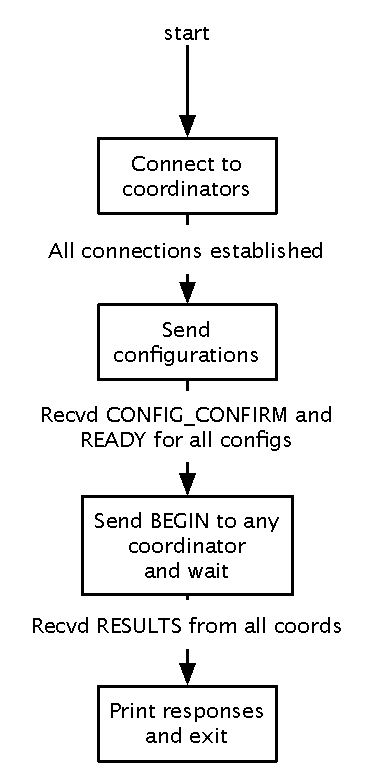
\includegraphics[scale=0.5]{figures/state_master.pdf}
    \end{center}
    \caption{State transition diagram for the master process.}
    \label{master}
\end{figure*}

To start the simulation, the master process sends \texttt{BEGIN} to any coordinator. It then waits for all coordinators to report back to it with information about the end of the simulation (RESULTS). Finally, it prints all relevant results.

A state transition diagram of this process is shown in figure \ref{master}.

\subsection{Coordinator}

The coordinator is the most complex part of the system. At any given time, as many as four threads may be running simultaneously. The full state transition diagram is shown in figure \ref{coord}.

At the high level, the coordinator connects to neighbors and agents, serves requests for information about the state of its agents in the last turn, and processes its own agents by requesting information from its neighbors and from its agents. In this way, the coordinators operate in lock-step, turn by turn, until all turns have been processed by all coordinators.

\subsubsection{The main thread}

The main thread handles the lifecycle of the coordinator and those of its connections. It begins by listening for a TCP connection from the master process. Once connected, it reads its configuration, which contains IP addresses/ports at which its neighbors are listening for it, which agents it should launch, and where to place them. It sends \texttt{CONFIG\_CONFIRM} back to the master process.

Coordinators are connected to each neighbor by two TCP connections. The coordinator listens on one of these for requests for information from the neighbor. It uses the other to request information of the neighbor. These connections are established using information sent from the master process.

Coordinators are connected to actors by a single TCP connection. To begin the agent communication process, the coordinator launches the agent process and repeatedly tries to open a socket to it until it responds.

The connections to the neighbors and agents are all established at once, asynchronously. When all connections are established, the coordinator sends READY to the master process and launches the \texttt{listenMaster} and \texttt{listenPeers} threads.

It waits for two locks, \texttt{TCOMPLETE1} and \texttt{TCOMPLETE2}, to be released. After these locks are released, the coordinator sends information about the final state of its agents back to the master process and exits, sending exit messages to the agents as well.

\begin{figure*}
    \begin{center}
        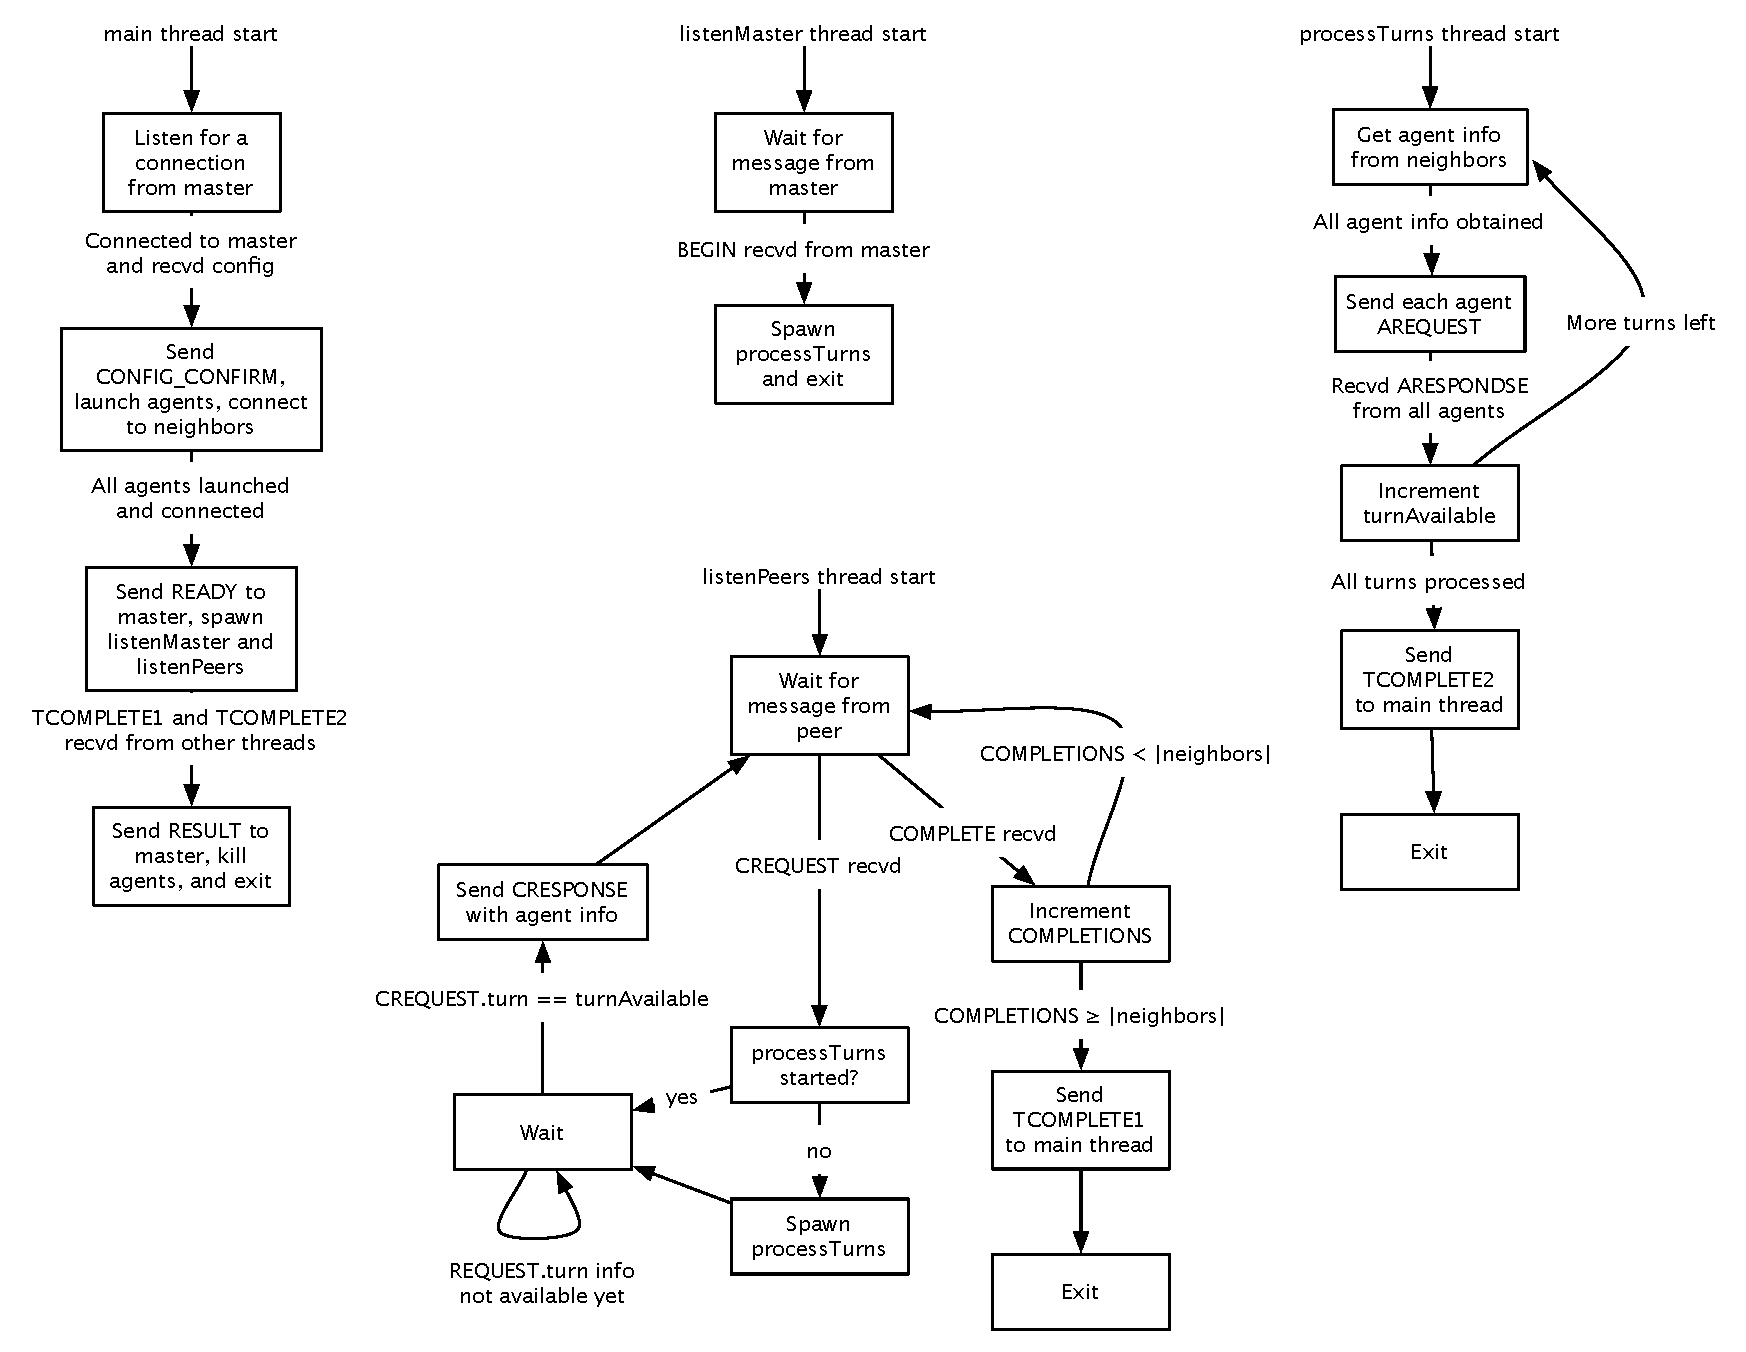
\includegraphics[scale=0.5]{figures/state_coord.pdf}
    \end{center}
    \caption{State transition diagram for the coordinator processes.}
    \label{coord}
\end{figure*}

\subsubsection{The listenMaster thread}

The master process begins the simulation by sending \texttt{BEGIN} to any coordinator. This message is received by the \texttt{listenMaster} thread, whose only job is to spawn the \texttt{processTurns} thread and exit.

\subsubsection{The listenPeers thread}

When \texttt{listenPeers} is spawned, all connections to neighbors have been set up. This thread listens for requests on its \textbf{incoming} connections (one for each neighbor).

When it receives a \texttt{CREQUEST} message containing the identifier of the requester, it sends back a \texttt{CRESPONSE} containing information about all of its agents that are relevant to the requester. (If agents are assigned to coordinators based on regions, then a neighbor does not need information about all of the coordinator's agents if some are far away.)

Additionally, if the \texttt{processTurns} thread has not been spawned when a \texttt{CREQUEST} is received, then it is spawned because some other coordinator must have been sent \texttt{BEGIN} by the master.

When sending \texttt{CRESPONSE} messages, the coordinator must be sure that it is sending information about the correct turn. To ensure this, a \texttt{turn} value is sent in the request and \texttt{listenPeers} blocks until the requested turn has been processed.

When the \texttt{listenPeers} thread receives a \texttt{COMPLETE} message, it increments an internal counter. When the counter is equal to the number of its neighbors, it unlocks \texttt{TCOMPLETE1} and exits.

\subsubsection{The processTurns thread}

This thread is responsible for handling interactions with agents. To execute a turn, it begins by sending \texttt{CREQUEST} messages to its neighbors to find out about relevant nearby agents that it does not have direct control over. Then it sends \texttt{AREQUEST} messages to each agent and awaits their \texttt{ARESPONSE} responses. It resolves the actions taken by the agents, including eliminating them from the grid, and informs \texttt{listenPeers} that the new turn has been processed.

The process repeats until all turns have been processed, at which point \texttt{TCOMPLETE2} is unlocked and \texttt{processTurns} exits.

\subsection{Agent}

\begin{figure*}
    \begin{center}
        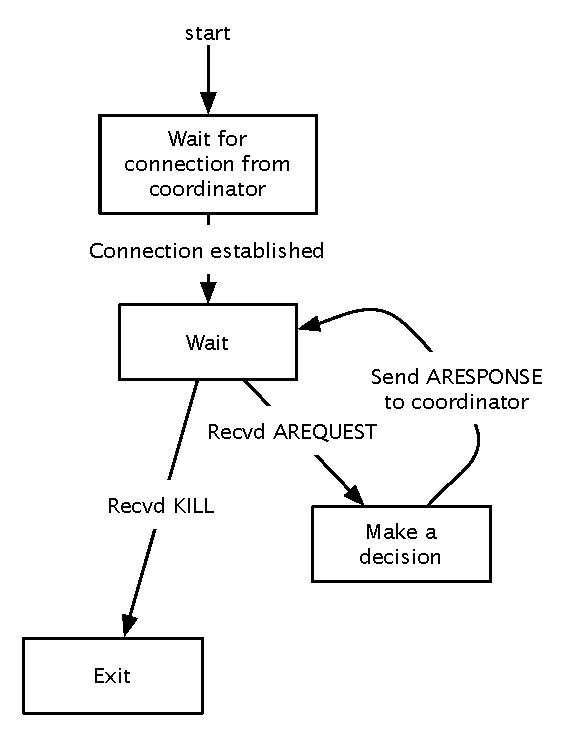
\includegraphics[scale=0.5]{figures/state_agent.pdf}
    \end{center}
    \caption{State transition diagram for the agent processes.}
    \label{agent}
\end{figure*}

The agent protocol is the simplest of all protocols defined for the system. It launches and waits for a connection from the coordinator, then repeatedly serves decision requests until told to exit.

\subsection{Discussion}

\subsubsection{Efficiency}

Consider a system with $|C|$ coordinators, $N$ neighbors per coordinator, $T$ turns, and $|A|$ agents. The master process sends $|C|$ messages (configurations) and receives $3|C|$ messages (two confirmations and one result per coordinator). The coordinators send $2N*T$ messages among themselves. Each coordinator also sends and receives one message per agent per turn, $|A|*T$. The total number of messages sent, therefore, is $4|C|+T(2N+|A|)$.

The size of half the messages sent between the coordinators, the \texttt{CRESPONSE} messages, are proportional to $|A|$ in the worst case, so the worst-case number of bytes sent is proportional to $4|C|+T(N+|A|(N+1))$. This is a truly degenerate case, however, so the equation in the previous paragraph is roughly accurate.

Since the number of messages grows linearly with respect to any individual variable, it meets the scalability requirements of the project.

\subsubsection{Stability}

The first versions of the protocols do not focus on stability, so they are vulnerable to crashes and corruption. There are no allowances for crashed processes. If the master process crashes, the coordinators will finish and then attempt to report their results. If a coordinator crashes, the rest of the coordinators will crash as well as they try to communicate with broken sockets. The agents will be left running, since they will never be told to die. If an agent crashes, the coordinator will crash along with it, causing the whole system to fall.

Since the simulation is deterministic, restarting the system on crash is not a terrible fate.
